\documentclass[main.tex]{subfiles} % Subfile-Class


% ============================================================================== %
%                            Subfile document                                    %
% ============================================================================== %

\begin{document}

% Template

\subsection{Organisation}

Das Projektteam ist agil organisiert. Die Idee ist, dass jedes Teammitglied
seine Verantwortung und den Zuständigkeit für eine bestimmte Teilfunktion des
Gerätes inne hat. Die entsprechenden Inkremente der Entwicklung werden jeweils
Freitags den anderen Teammitgliedern vorgestellt und in der offenen Runde
diskutiert. Dabei wird sichergestellt, dass wichtige Weichen für
Schnittstellen, beispielsweise Mechanische Umsetzung mit Elektrischer
Ansteuerung, frühzeitig gestellt werden und bei auf kommenden Problemen auch
früh reagiert werden kann. Darüber hinaus sind noch Ämter verteilt wie die
allgemeine Organisation, Mechanik-Werkstatt-Beauftragter sowie die
Budgetplanung.

Abbildung~\ref{fig:Organigramm} zeigt eben diese Struktur des Teams.

\begin{figure}[h!]
    \centering
    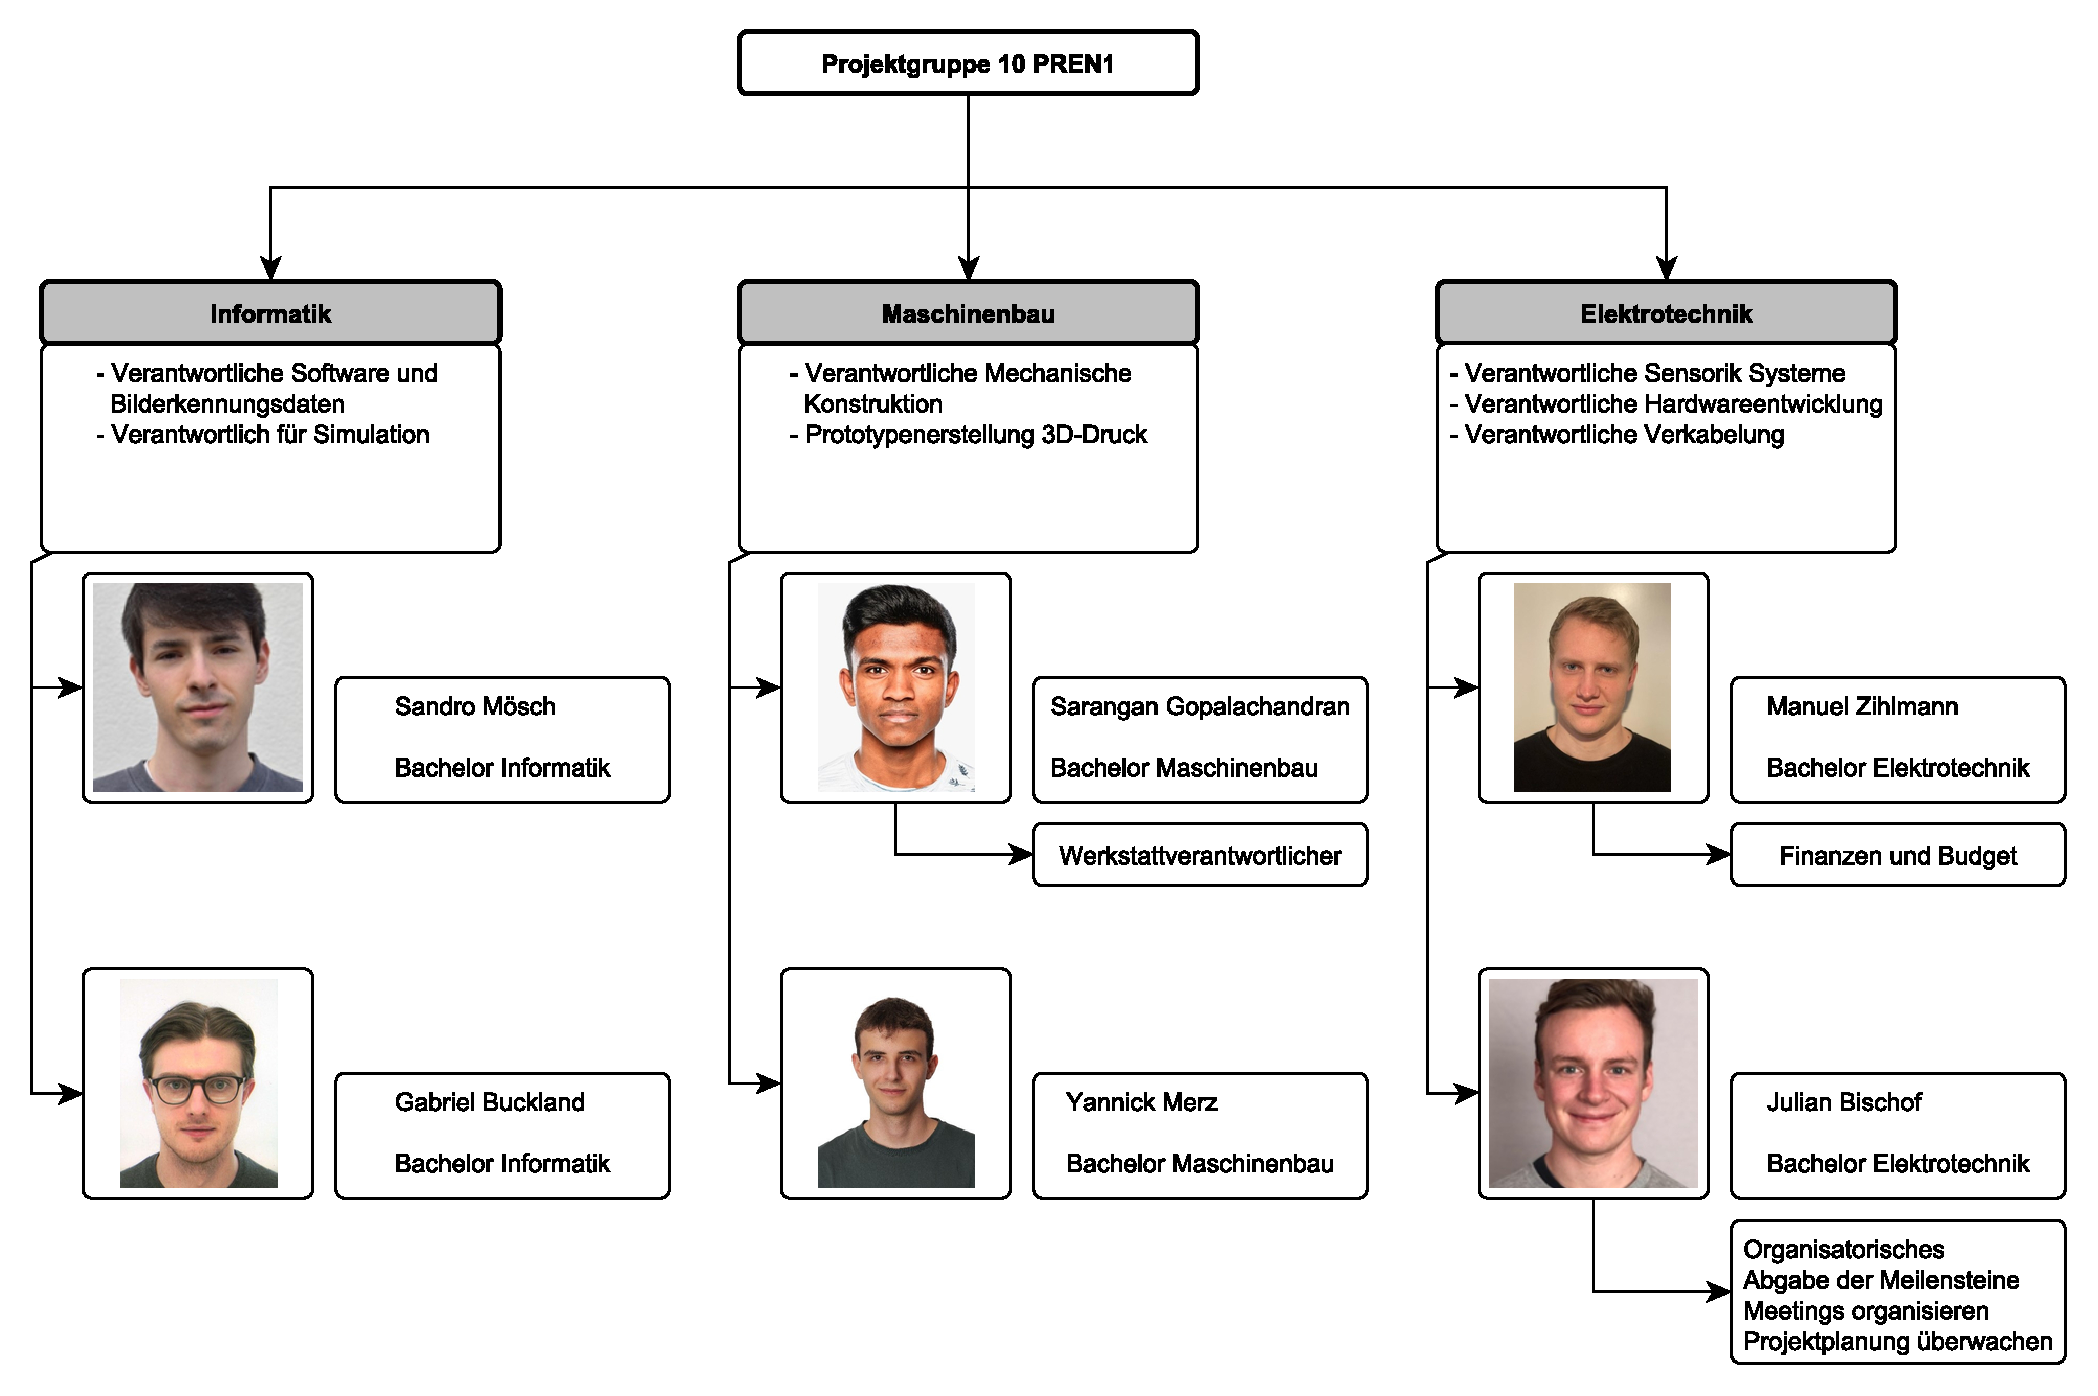
\includegraphics[page=1, width=1\textwidth]{./fig_Projektmanagement/Organigramm.pdf}
    \caption{Organigramm Team 10}\label{fig:Organigramm}
\end{figure}

\end{document}
